%%% Installations
Afin de pouvoir programmer votre module Arduino Nano, plusieurs étapes sont nécessaires.

Il vous faut d'abord \textbf{télécharger et installer le programmateur Arduino}. Celui-ci est aussi appelé Arduino IDE (Arduino Integrated Development Environment). Voici les instructions à suivre :
\begin{enumerate}
	\item se rendre sur la page principale du site Arduino (\url{www.arduino.cc/}) ;
	\item cliquer sur l'onglet "Software > Downloads" ; 
	\item choisir votre version d'Arduino IDE (voir Fig. \ref{fig:arduino_ide}) et la télécharger ;
	\item une fois le téléchargement effectué, il ne vous reste plus qu'à installer le programmateur.
\end{enumerate}

\begin{figure}[ht!]
	\centering
	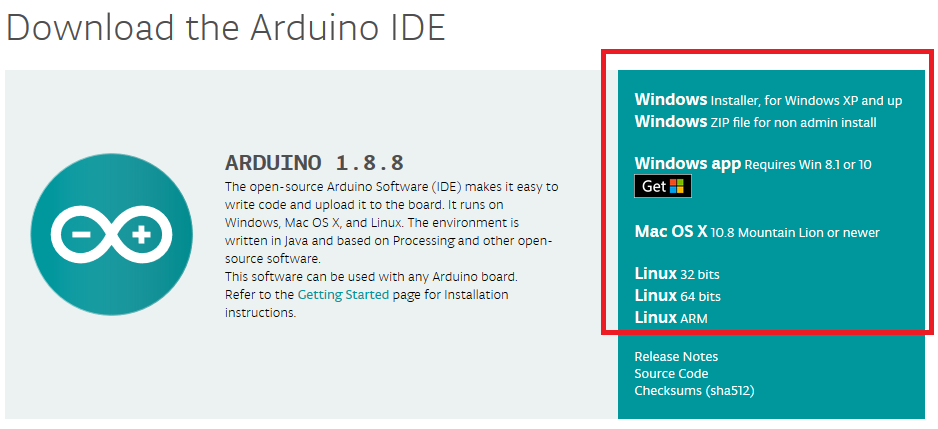
\includegraphics[width=\textwidth]{imgs/arduino_ide.png}
	\caption{Téléchargement du programmateur Arduino.}
	\label{fig:arduino_ide}
\end{figure}

Pour la suite de la séance, il vous faudra également \textbf{installer la librairie IRremote}. Cette librairie gère l'interfaçage avec le récepteur infrarouges et permettra à votre Arduino Nano de correctement recevoir les données envoyées par la télécommande infrarouges. Voici les instructions à suivre :
\begin{enumerate}
	\item ouvrir l'Arduino IDE fraichement installé ;
	\item aller dans \textit{Sketch --> Include Library --> Manage Libraries...} ;
	\item taper "IRremote" dans la barre de recherche ;
	\item cliquer sur la librairie "IRremote" (voir Fig. \ref{fig:arduino_IRremote}) et l'installer ;
	\item voilà ! 
\end{enumerate}

\begin{figure}[ht!]
	\centering
	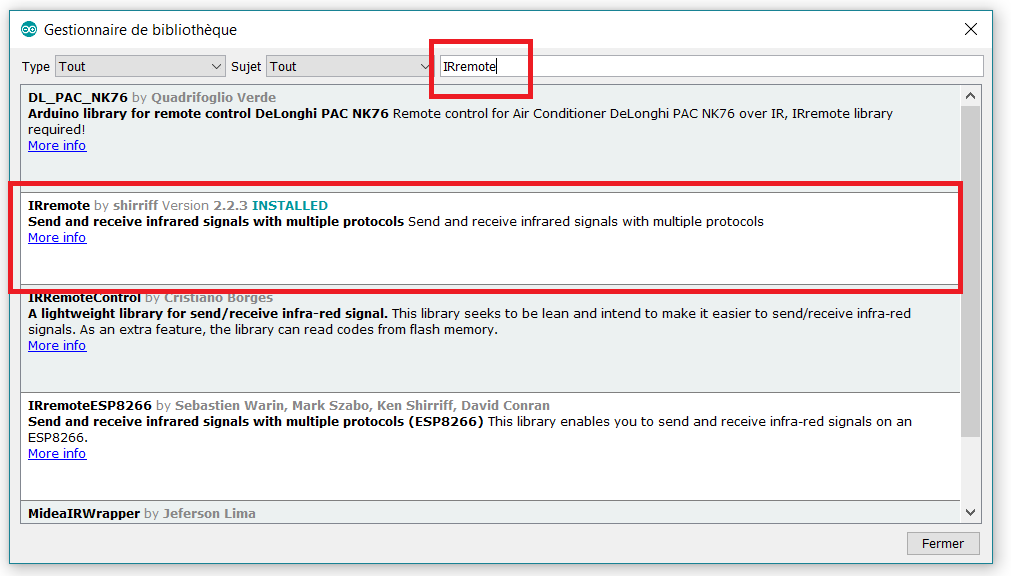
\includegraphics[width=\textwidth]{imgs/arduino_IRremote.png}
	\caption{Installation de la librairie IRremote.}
	\label{fig:arduino_IRremote}
\end{figure}

Enfin, avant de programmer votre module Arduino, il faut s'assurer que certaines configurations soient bien faites dans l'IDE Arduino: d'abord le type de module Arduino que nous allons programmer (Nano dans notre cas), ensuite le type de processeur existant sur ce module (ATmega328P dans notre cas). Voici comment faire pour choisir ces paramètres:
\begin{enumerate}
	\item aller dans \textit{Tools --> Board} et choisir \textit{Arduino Nano} comme type de module Arduino à utiliser (voir Figure \ref{fig:arduino_board}).
	\item aller dans \textit{Tools --> Processor} et choisir \textit{ATmega328P} comme processeur (voir Figure \ref{fig:arduino_processor}).
\end{enumerate}

\begin{figure}[ht!]
	\centering
	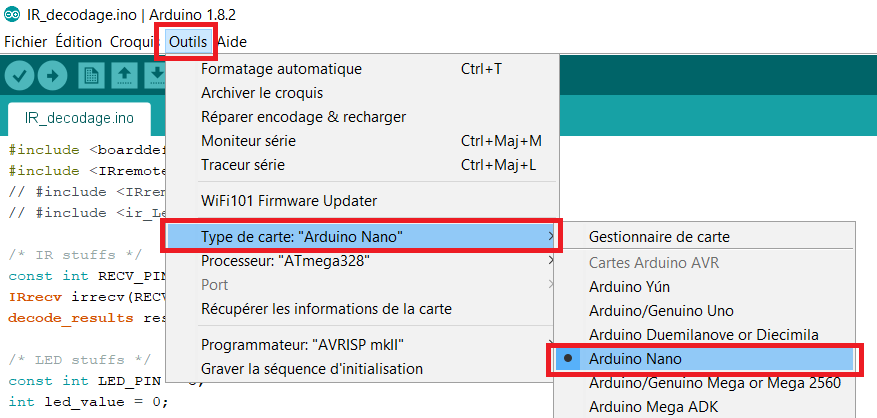
\includegraphics[width=\textwidth]{imgs/arduino_board_v2.png}
	\caption{Choix du type de module Arduino.}
	\label{fig:arduino_board}
\end{figure}

\begin{figure}[ht!]
	\centering
	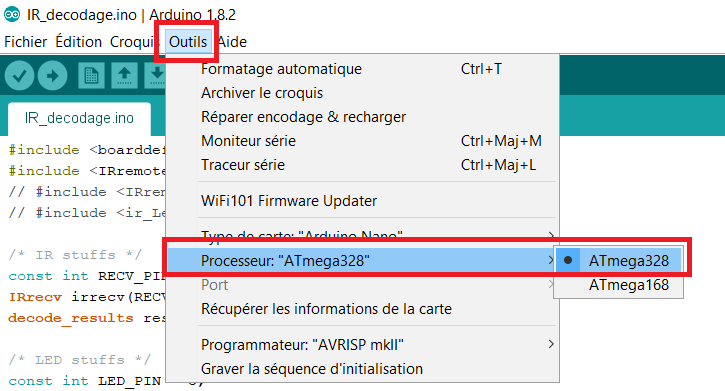
\includegraphics[width=\textwidth]{imgs/arduino_processor_v2.png}
	\caption{Choix du type de processeur sur le module Arduino.}
	\label{fig:arduino_processor}
\end{figure}

Vous êtes enfin prêts à programmer votre module Arduino. Vous l'aurez remarqué, Arduino est open-source et gratuit. Sachez aussi qu'il existe une floppée de librairies existantes pour faire à peu près n'importe quoi !









%Les moteurs utilisés pour ce projet sont des moteurs DC à balais. Ce type de moteur ne nécessite qu'une source de tension DC pour l'alimenter, au contraire de moteurs synchrones ou asynchrones, basés sur des alimentations triphasées ou N-phasées.\\
%
%\begin{minipage}[t]{.45\textwidth}
%	\centering
%	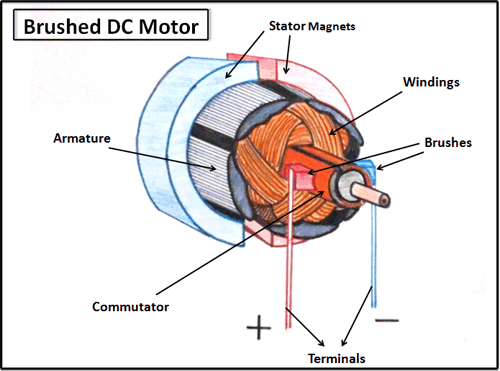
\includegraphics[width=\textwidth]{dc_motor}
%	\captionof{figure}{Schéma d'un moteur DC.}
%	\label{fig:dc_motor}
%\end{minipage}
%\hfill
%\begin{minipage}[t]{.45\textwidth}
%	\centering
%	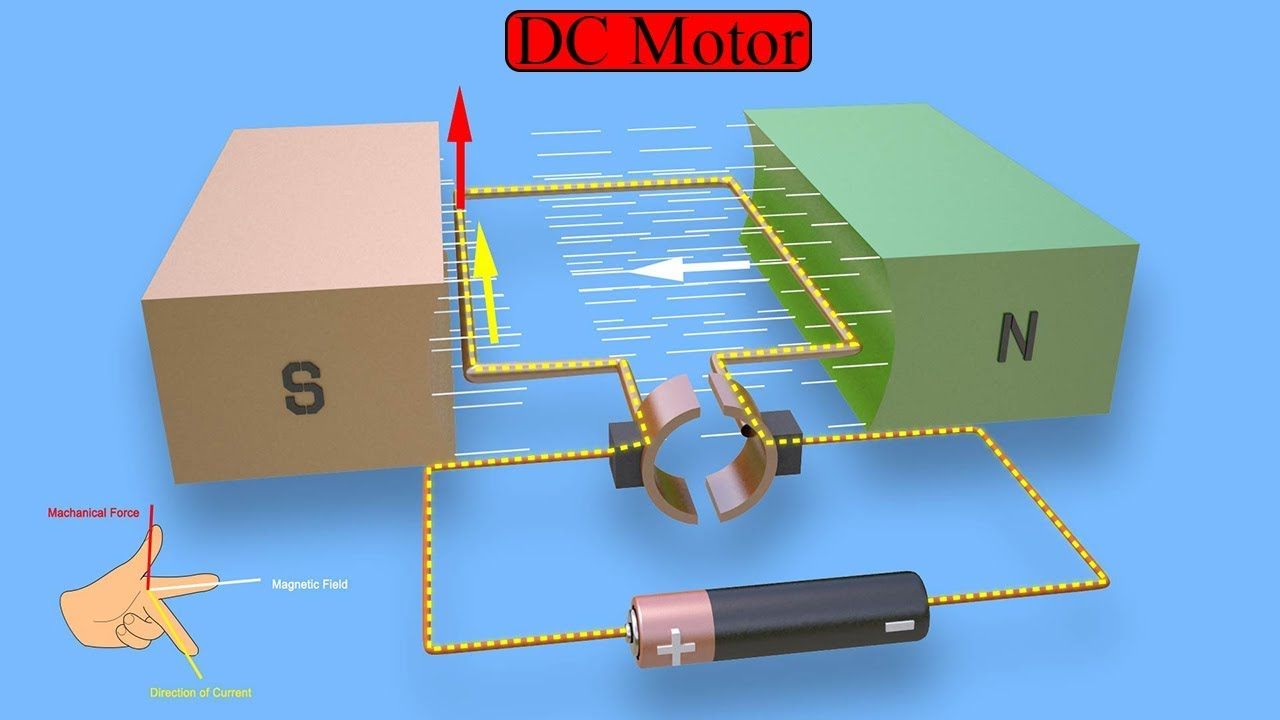
\includegraphics[width=\textwidth]{dc_motor_principle}
%	\captionof{figure}{Principle de fonctionnement du moteur DC.}
%	\label{fig:dc_motor_principle}
%\end{minipage}
%\vspace{.25cm}
%
%Le moteur est constitué de deux pièces principales, comme illustré à la Figure \ref{fig:dc_motor}. D'une part, un \textbf{stator}, élément fixe du moteur, sur lequel on trouve généralement une structure formée d'aimants permanents, servant à générer un champ magnétique de direction fixe. D'autre part, un \textbf{rotor}, élément mobile du moteur, sur lequel on trouve généralement des bobinages alimentés par la tension DC fournie au moteur, servant à générer un champ magnétique de direction variable.\\
%
%Le couple électro-mécanique produit par le moteur résulte du moment de force qui tend à aligner les directions des champs magnétiques générés respectivement par les aimants permanents au stator et les bobinages au rotor, comme représenté à la Figure \ref{fig:dc_motor_principle}. Un commutateur auquel les bobinages sont connectés au travers d'un système de balais, permet de choisir quels bobinages alimenter, de façon à constamment désaligner le champ magnétique résultant des bobinages par rapport à celui des aimants. C'est ce principe qui permet de produire un mouvement rotatif continu.\\
%
%D'un point de vue purement électrique (et pour votre information uniquement, pas besoin de comprendre les détails), le fonctionnement du moteur DC est régi par 2 équations principales:
%
%\begin{align*}
%	\left \lbrace
%	\begin{aligned}
%		V_a &= R_a I_a + L_a \frac{dI_a}{dt} + k \phi \omega_m\\
%		C_{em} &= I \frac{d\omega_m}{dt} = k \phi I_a
%	\end{aligned}
%	\right. 
%\end{align*}
%
%La \textbf{première équation} relie la tension d'alimentation du moteur, notée $V_a$, au courant circulant dans les bobinages, noté $I_a$ et à la force électromotric induite (le terme $k \phi \omega_m$) qui fait directement intervenir la vitesse de rotation du moteur $\omega_m$. La \textbf{seconde équation} relie le couple électro-mécanique, noté $C_{em}$ et proportionel à la dérivée de la vitesse de rotation $\frac{d\omega_m}{dt}$, au courant dans les bobinages.\\
%
%La conclusion principale à tirer de ces équations est qu'il est possible de contrôler la vitesse du moteur $\omega_m$ uniquement en modulant la tension $V_a$ appliquée au moteur.